\chapter{序論}

\section{研究背景}
スマートタグとは貴重品などに取り付け, 紛失した際に捜索を補助するデバイスである. 
補助の方法はタグが音を鳴らす方法と付近のスマートフォンと無線通信する方法が一般的である. 
近年こうした製品が普及しており, なくしものの対策に需要があることを示唆している. 
しかし特性上タグの取り付けが困難な物もある. 
例えば入れ歯は口内で使用するために衛生や防水, 日常生活の邪魔になるなどの理由で取り付けが難しい. 

\section{関連研究}
タグを必要としないなくしもの対策として, 草野\index{くさの@草野}らは家庭内での移動マニピュレータによるベイズ推定と自然言語処理を用いた物品捜索手法を提案している. \cite{kusano}
この手法は捜索範囲を小領域に区切り, 捜索した履歴から小領域ごとにベイズ推定により捜索対象がある確率を計算し, 確率が最大の小領域から順に捜索するものである. 
また確率が最大の小領域が複数ある場合は, 自然言語処理により小領域内の家具と捜索対象の関連も考慮する. 

\begin{figure}[H]
    \begin{center}
        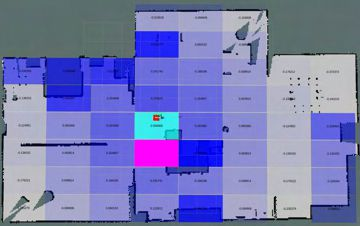
\includegraphics[width=0.8\linewidth]{figs/kusano.jpg}
        \caption{Existence probability of target object}
        \label{fig:kusano}
    \end{center}
\end{figure}

なくしものは発生頻度が低いため, 利用者への最適化が進みづらいことが想定される. 

\section{研究目的}
利用者の普段の行動を反映することで最適化がより進む
確率論でモデル化
なくしものの位置の確率分布を計算
